\documentclass[11pt, letterpaper]{article}

\usepackage[margin=1in]{geometry}
\usepackage[utf8]{inputenc}
\usepackage{datetime}
\usepackage{latexsym}
\usepackage{amsfonts,amssymb,amsmath}
\usepackage{booktabs, array}
\usepackage{xcolor}
\usepackage{graphicx}
\graphicspath{../images/}
\usepackage{float}

\usepackage{textcomp}

\usepackage{tocloft}
\renewcommand{\cftsecleader}{\cftdotfill{\cftdotsep}}  % for Sections




\usepackage{hyperref}
\hypersetup{
	colorlinks = true,
	linkcolor={blue!80!black},
	citecolor={blue!80!black},
	urlcolor={blue!80!black}}
%\usepackage{Sweave}
\begin{document}
%\input{Report-concordance}



\title{"Monte Carlo Simulation of Lockout From Multiple Data Centers"}
\author{"Nicholas Lauerman"}
\date{}

\begin{abstract}
\addcontentsline{toc}{section}{Abstract}
Abbott has a requirement that a user account be locked out after 10 failed login
attempts. This paper is a Monte Carlo simulation of this were the failed attempts
is not tracked by user but by user at each data center
\end{abstract}

\tableofcontents
\listoffigures
\listoftables

\section{Background}
For a recent release of CHaRM
\footnote{CHaRM - Complaint Handling and Risk Management System}
the requirement that a user be locked out after ten failed 	attempts
\footnote{Per procedure 4-010-001} was tested. This test failed, this
feature is managed through Active Directory (AD) so a the issues was
elevated to the AD team within BTS. It was determined that AD was
functioning as required after BTS raised a ticket with
Microsoft\texttrademark which replied that the system was working as
expected due to the ``Smart Logout'' feature. Along with issues in how it
counts attempts the failed attempts are only counted at each data center,
but each request is independently routed to different data centers
depending on 	load and something called ``geo-distributed.''

\subsection{Assumptions}
This simulation is based on the following assumptions.
\begin{enumerate}
\item That there are 47 Azure (Microsoft cloud) data centers.
Recent Microsoft advertising indicated that there are 47 data centers
or backup locations supporting Azure. The specific assumption is
that there are no stand-alone backup location but one data center
serves as a backup location for one or more other data centers.
\item That any log-in attempt will have an equal chance to be
assigned to any available data center
\item That the only impact on the number of attempts prior to lockout is
from the counting of failed log-in attempts at the individual data centers. Even though
this is a significant impact there are other factors in the "Smart Logout" feature
that would potentionally increase the total log in attempts.
\item That the random number generator has sufficient entropy for
the purpose of this simulation.
\end{enumerate}

\subsection{Method}
Each simulation run will consist of a data center being selected and the
failed counter incremented then check to see if that counter has reached
ten, what is considered a lock out. the number of attempts is them report
for that run. A run will be repeated multiple times and the average and
other data will be computed. These simulations will be run multiple times in an
attempt to reflect actual behavior.


\section{Simulations}
\subsection{Two Data Centers}
The first simulation will be a simple case with mininual data centers. This will
show the impact of the added data center.

\begin{table}[H]
	\centering
	\caption{Simulation Parameters --- First Simulation}
	\begin{tabular}{||r|l||}
		\hline \hline
		Parameter & Value \\ \hline \hline
		Data Centers & 2 \\ \hline
		Simulation Runs & 1,000 \\ \hline \hline
	\end{tabular}
	\label{tab:Sim1_set}
\end{table}


\subsubsection*{Results}
\begin{table}[H]
	\centering
	\caption{Simulation Results --- First Simulation}
	\begin{tabular}{||r|l||}
		\hline \hline
		Result                  & Value                     \\ \hline \hline
		Mean                    & 16.357    \\ \hline
		Standard Deviation      & 1.98632738905159    \\ \hline
		Median                  & 17    \\ \hline
		Maxinum                 & 19    \\ \hline
		Minimum                 & 10    \\ \hline \hline
	\end{tabular}
	\label{tab:Sim1_res}
\end{table}

\begin{figure}[H]
\centering
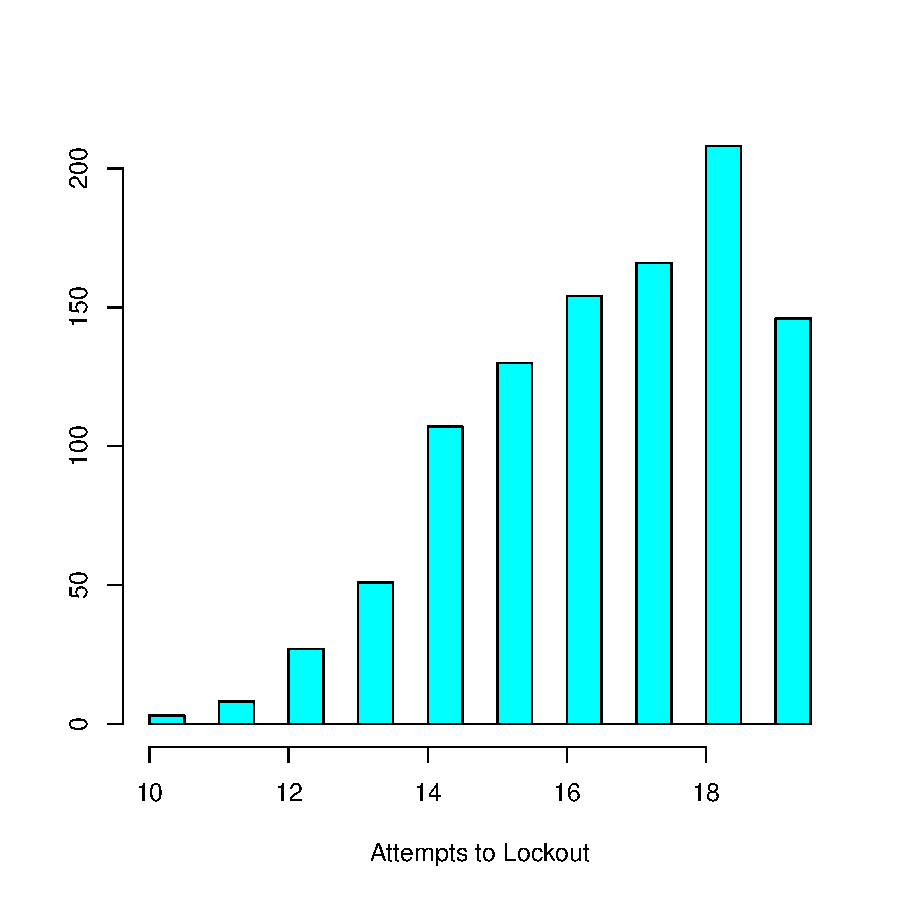
\includegraphics{Report-003}
	\caption{Histogram for 2 data centers}
	\label{fig:hist_1}
\end{figure}

\subsection{Worse case}
This simulation will be for the worse case with 47 data centers hosting Abbott's
Activity Directory

\begin{table}[H]
	\centering
	\caption{Simulation Parameters --- Second Simulation}
	\begin{tabular}{||r|l||}
		\hline \hline
		Parameter & Value \\ \hline \hline
		Data Centers & 47 \\ \hline
		Simulation Runs & 1,000 \\ \hline \hline
	\end{tabular}
	\label{tab:Sim2_set}
\end{table}


\subsubsection*{Results}
\begin{table}[H]
	\centering
	\caption{Simulation Results --- Second Simulation}
	\begin{tabular}{||r|l||}
		\hline \hline
		Result                  & Value                     \\ \hline \hline
		Mean                    & 16.357    \\ \hline
		Standard Deviation      & 1.98632738905159    \\ \hline
		Median                  & 17    \\ \hline
		Maxinum                 & 19    \\ \hline
		Minimum                 & 10    \\ \hline \hline
	\end{tabular}
	\label{tab:Sim2_res}
\end{table}

\begin{figure}[H]
\centering
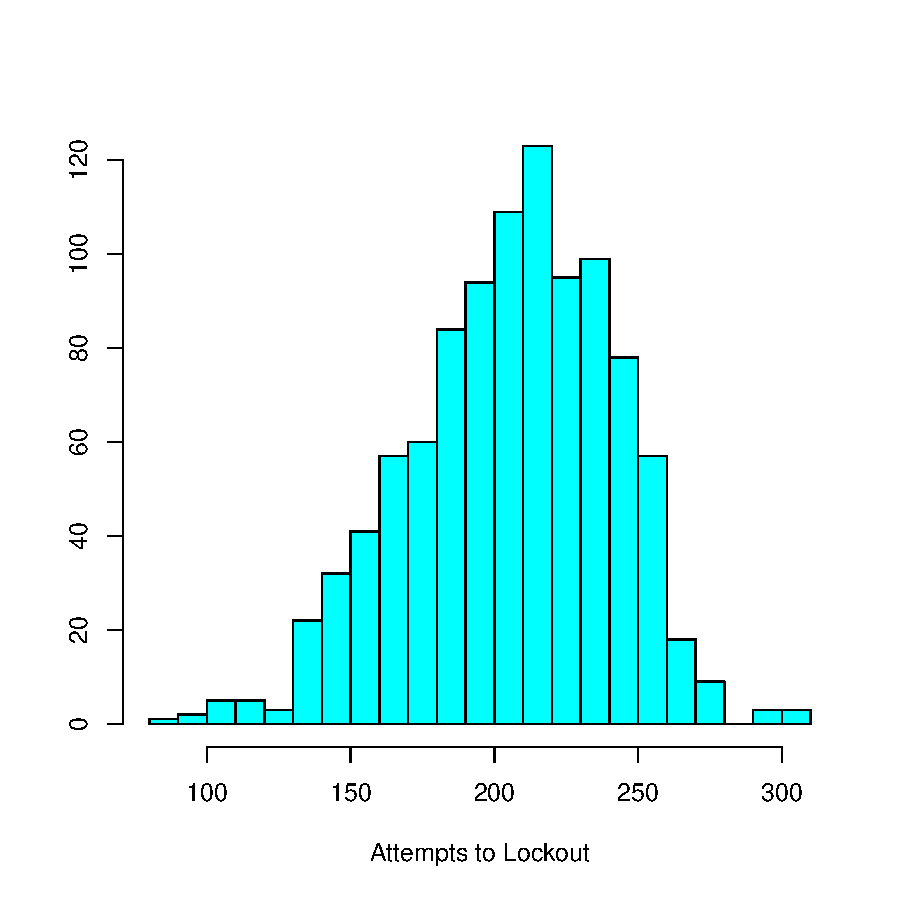
\includegraphics{Report-005}
	\caption{Histogram for 47 data centers}
	\label{fig:hist_2}
\end{figure}

\subsection{Projection of number of attempts}
This graph shows the average number of attempts for data center
with a minimum of 2 and a maximum of 47. It also shows a linear
fit to the data along with the range for the 99.9\% confidence interval. Finally,
it shoes the theoritical maximun and the required number (10).

\begin{table}[H]
	\centering
	\caption{Simulation Parameters --- Third Simulation}
	\begin{tabular}{||r|l||}
		\hline \hline
		Parameter & Value \\ \hline \hline
		Data Centers & 2 to 47 \\ \hline
		Simulation Runs & 1,000 \\ \hline \hline
	\end{tabular}
	\label{tab:Sim3_set}
\end{table}



\begin{figure}[H]
\centering
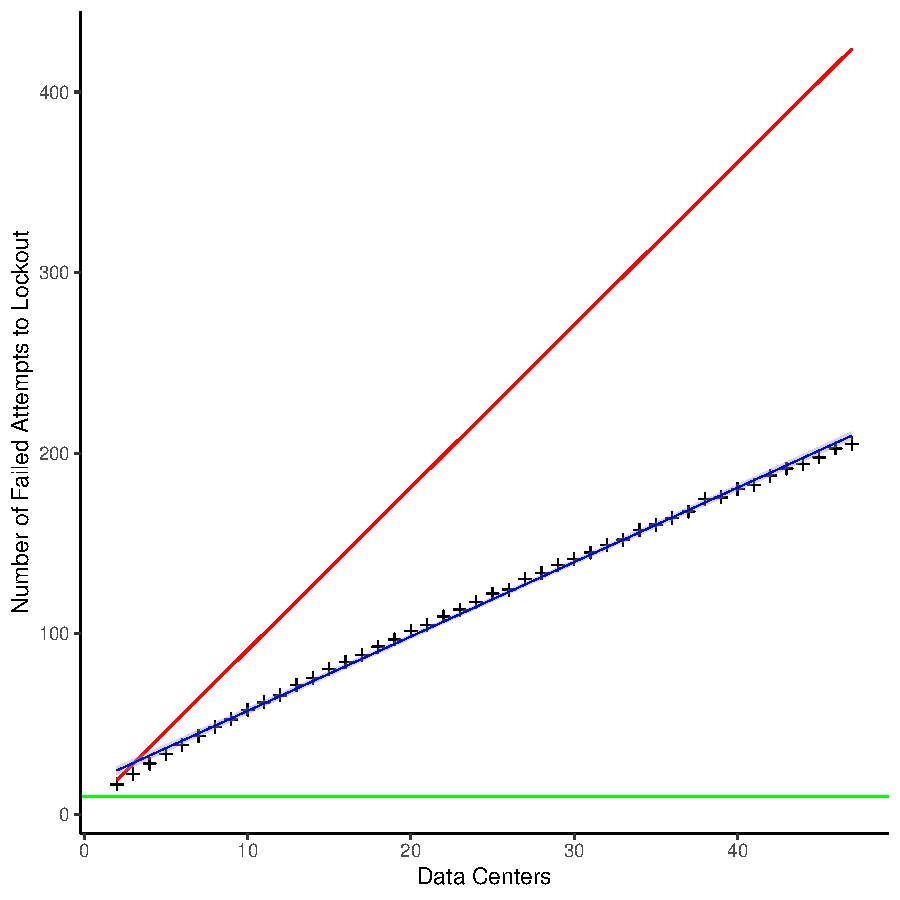
\includegraphics{Report-007}
	\caption{Garph showing prodicted number of attempts for lockout for up to 47
	data centers}
	\label{fig:plot_3}
\end{figure}

\subsection{Projection of number of attempts, first ten}
This graph shows the average number of attempts for data center
with a minimum of 2 and a maximum of 10. This is a new simulation as well that
shows that the simulation results are simular between runs. The graph also shows a linear
fit to the data along with the range for the 99.9\% confidence interval. Finally,
it shoes the theoritical maximun and the required number (10).

\begin{table}[H]
	\centering
	\caption{Simulation Parameters --- Fourth Simulation}
	\begin{tabular}{||r|l||}
		\hline \hline
		Parameter & Value \\ \hline \hline
		Data Centers & 2 to 10 \\ \hline
		Simulation Runs & 1,000 \\ \hline \hline
	\end{tabular}
	\label{tab:Sim4_set}
\end{table}



\begin{figure}[H]
\centering
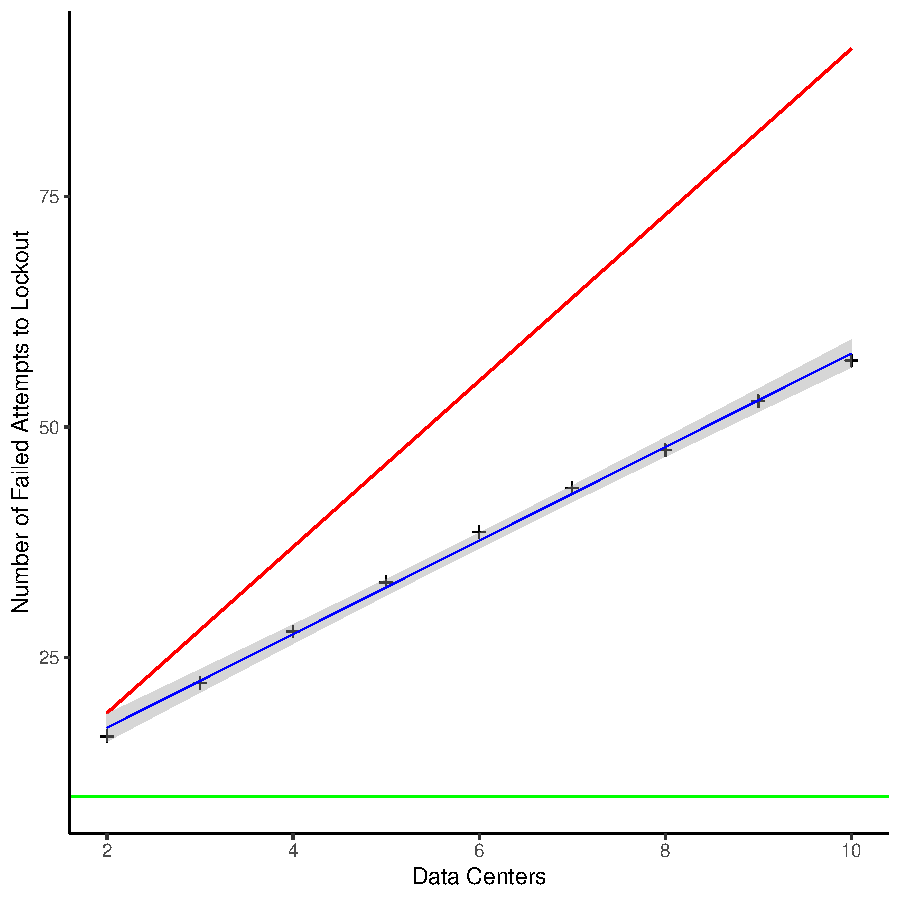
\includegraphics{Report-009}
	\caption{Garph showing prodicted number of attempts for lockout for up to 10
	data centers}
	\label{fig:plot_4}
\end{figure}



\end{document}
